\setcounter{subsection}{0} 
In this chapter, the main features of the Electromagnetic Calorimeter are explained, including the ECL reconstruction algorithm and the introduction of cluster variables.


\part{ECL chracteristics and cluster variables}
\subsubsection{The ECL reconstruction algorithm} 
For each ECL crystal, a 32-bit word is recorded as the digitized output from the electronics. This 32-bit word, referred to as \textbf{ECLDigit}, encodes: 
\begin{itemize}
\item energy information as Flash Analog-to-Digital Converter (FADC) counts (18 bits),
\item time information in clock ticks (12 bits),
\item 2 status bits (signal quality flags).
\end{itemize}
To reconstruct the shower, an algorithm processes the ECLDigit objects into two new data objects: 
\begin{itemize}
\item \textbf{ECLShowers}, an ECL-internal object containing additional  debug information,
\item \textbf{ECLClusters}, the primary analysis object.
\end{itemize}
Only ECLShowers with $E > 20$\ MeV are converted to ECLClusters.
$\\$
The first step identifies \textbf{connected regions}, which rapidly reduces the combinatorial complexity. These are specific cell collections determined by a dedicated clustering procedure. 
$\\$
An example of this procedure is shown in Fig.~\ref{fig:ECL_clustering_proc}.

\begin{figure}[H]
    \centering
    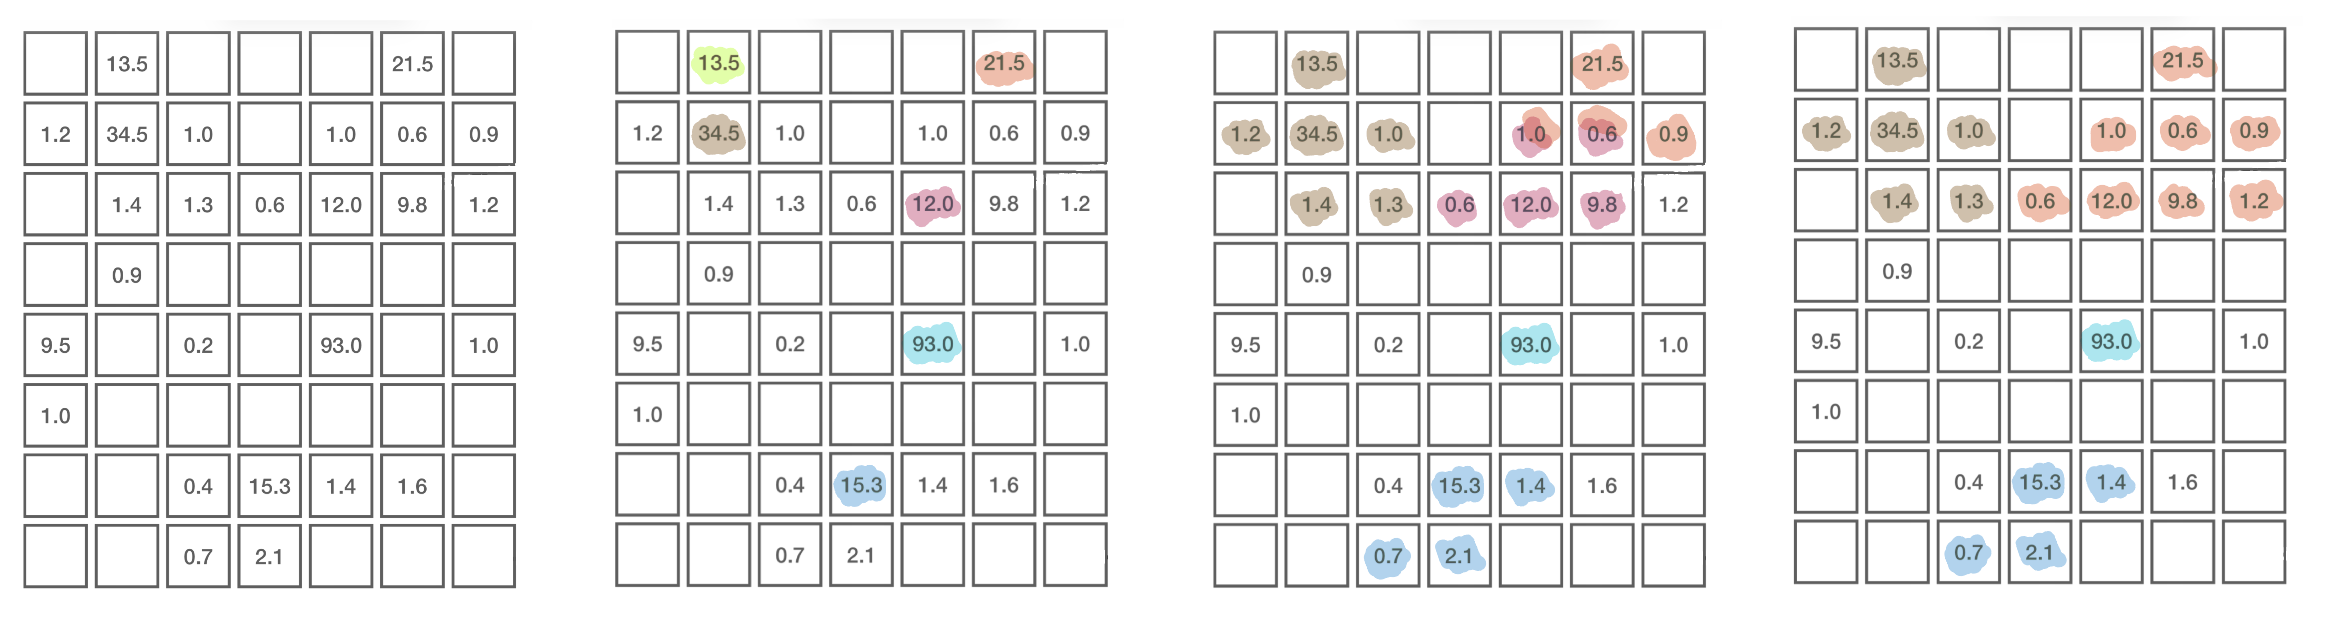
\includegraphics[width=1\textwidth]{belleII_det/images/ECL_algo}
  \caption{Description of ECL clustering process: (a) Step 0; (b) Step 1; (c) Step 2; (d) Step 3.}
  \label{fig:ECL_clustering_proc}
\end{figure}

Each cell represents one ECLDigit, with its value corresponding to the deposited energy in MeV. Empty cells indicate ECLDigit values below the readout threshold (0.1\,MeV in this example). 
$\\$
In step 1, every ECLDigit above 10 MeV is selected. In step 2, any neighbors above 0.5 MeV are attached to the highest-energy seed found in step 1. Sometimes two seeds compete for the same neighbor, and sometimes clusters have no neighbors (i.e. 93.0). In step 3, overlapping neighbor regions trigger a merge. Additionally, any cells above 1.5 MeV recruit their next neighbors iteratively.
$\\$
After this process, the connected regions are obtained, as shown in Fig.~\ref{fig:c_region}.
\begin{figure}[H]
    \centering
    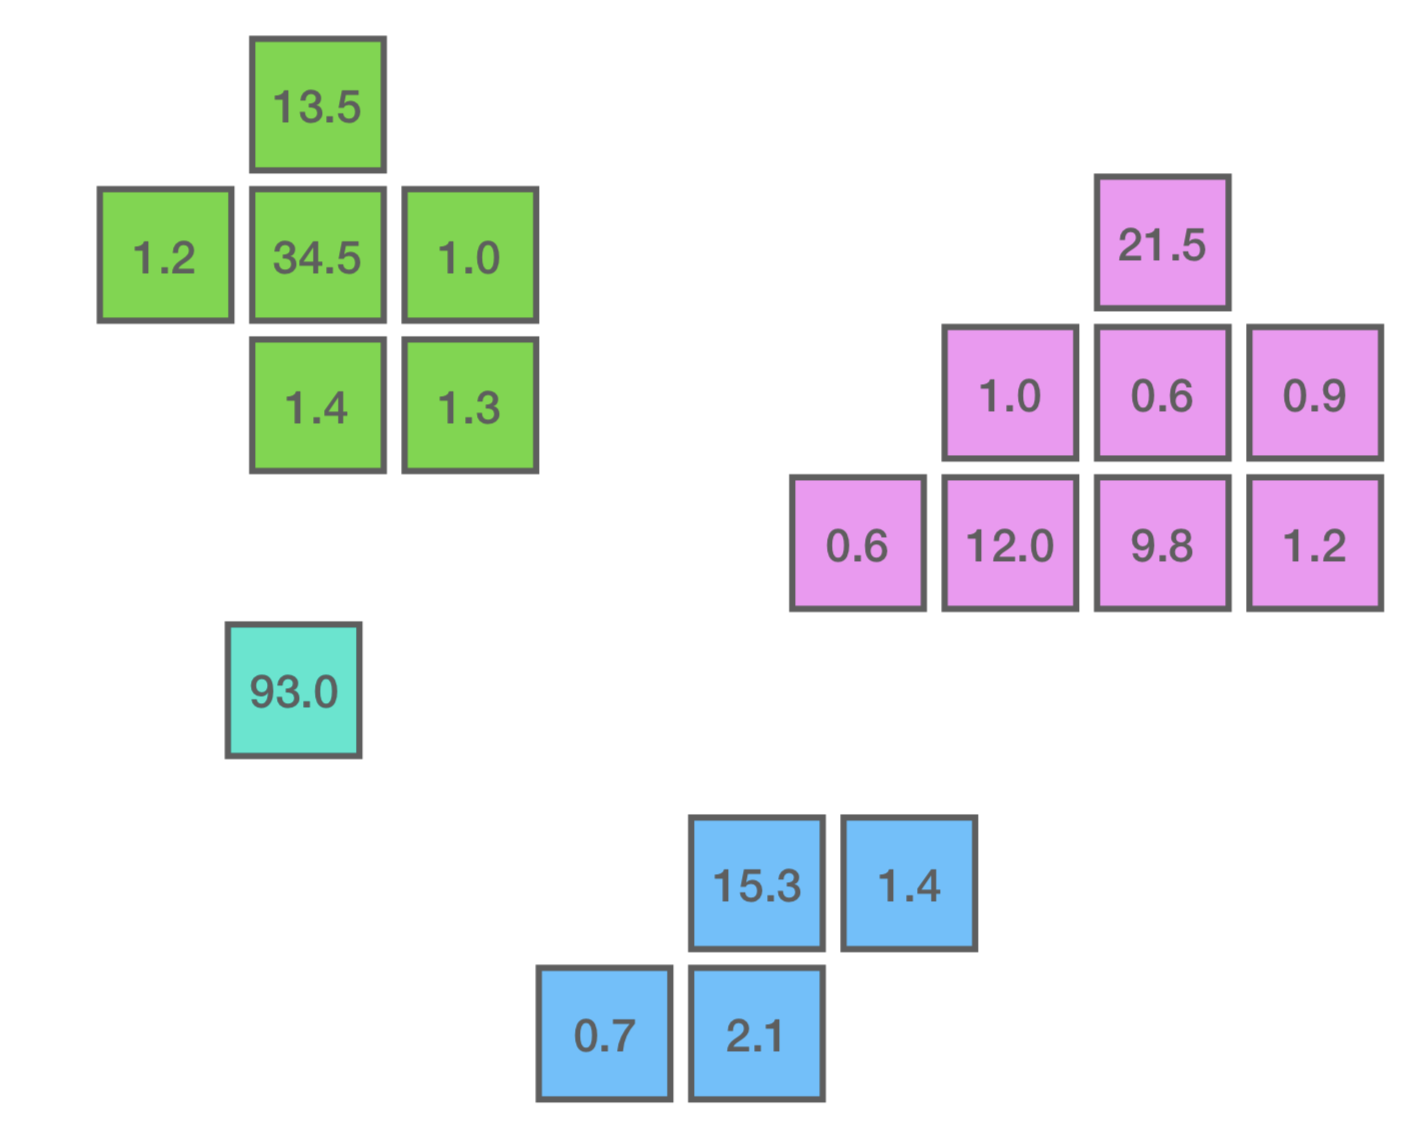
\includegraphics[width=0.5\textwidth]{belleII_det/images/ConnectedRegions}
    \caption{Connected regions obtained in the example (threshold: 0.1 MeV).}
    \label{fig:c_region}
\end{figure}
The final step is to pick the crystals with energy above 10 MeV, namely the Local Maxima (LM). Every connected region has one LM at least. The connected regions are furtherly processed in order to obtain the position and the energy of the cluster, processing the LM with a splitting-weighting process among the connected regions crystals \cite{denuccio2019}. 
$\\$
The main idea is that an ECLShower object is produced from every LM. If a connected region contains only one LM, the total energy of its crystals is assigned to the corresponding ECLShower. Otherwise, if multiple local maxima are present, an iterative procedure is performed, where the weight for each crystal depends on the distance of the crystal from the center-of-gravity of each ECLShower (center-of-gravity is calculated using weighted energies).
$\\$
Connected regions are used to minimize the number of times the computationally intensive splitting procedure must be performed.

\subsubsection{ECL performance}
The observed ECL \textbf{energy resolution} can be written as follow:
\begin{center}
$\frac{\sigma_E}{E} = \sqrt{ \left( \frac{0.81\%}{\sqrt[4]{E}} \right)^2 + \left( \frac{0.066\%}{E} \right)^2 + (1.34\%)^2 }$,
\end{center}
where the first term represents stochastic fluctuations (Poissonian statistics) in the shower generation, the second term accounts for electronic noise, and the third is a constant term dependent on calibration.
$\\$
For example, $\frac{\sigma_E}{E} = 4\%$ at 100 MeV and $\frac{\sigma_E}{E} = 1.4\%$ at 8 GeV \cite{abashian2002}). The energy resolution behavior is shown in Fig.~\ref{fig:ECL_sigmaE}.

\begin{figure}[H]
    \centering
    \includegraphics[width=1\textwidth]{belleII_det/images/energy-res}    
  \caption{The energy resolution as a function of incident photon energy for the (a) 3Y3 and (b) 5Y5 matrix with total energy sum. The error bars are not statistical but are the rms of four measurements taken with the crystals (3,3), (3,4), (4,3) and (4,4) into the photon beam \cite{ikeda2000belle}.}
  \label{fig:ECL_sigmaE}
\end{figure}

\subsection{Shower shape variables in the signal sample}
The following chapter introduces the core of this thesis: the analysis of the \textbf{shower shape variables} of neutral ECL clusters associated with anti-neutron candidates. Since the final goal is to assess Data/MC agreement for these variables, the shower shape variables are first studied in an MC signal sample with no background channels present. The main idea is that particle identification can be achieved by studying the shower shapes and their characteristics.

The selected variables are the \textbf{cluster energy}, the \textbf{E1E9} variable, the \textbf{E9E21} variable, \textbf{Lateral Momentum}, \textbf{Second Moment}, \textbf{Zernike Moments} (50 and 41), and \textbf{Number of Hits}, which are described first. 

\paragraph{Cluster Energy}
$\\$
The Cluster Energy (\emph{clusterE} in the basf2 software), as the name suggests, represents the total energy deposited by the cluster associated with a given candidate particle, in this case the anti-neutron. It has units of GeV and only clusters with Cluster Energy above 20 MeV are stored by the reconstruction software.

\paragraph{Cluster E1E9 and E9E21}
In order to provide a proper definition of these variables (respectively \emph{clusterE1E9} and \emph{clusterE9E21} in the basf2 software), the following figure is shown below:

\begin{figure}[H]
    \centering
     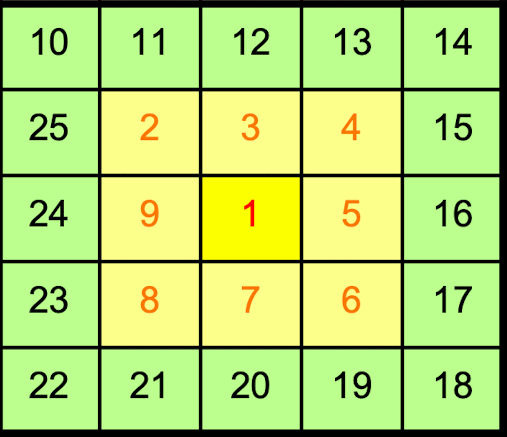
\includegraphics[width=0.50\textwidth]{nbar_MC/images/cluster}
     \caption{Ideal representation of a cluster pattern, consisting of a 5×5 matrix in which each cell corresponds to a single crystal}
\end{figure}

Cluster E1E9 and cluster E9E21 are defined as follow:

\begin{center}
$E1E9 = \frac{E_1}{\sum_{i=1}^{9} E_i}$ \hspace{0.2cm} $E9E21 = \frac{\sum_{j=1}^{9} E_j}{\sum_{j=10}^{25} E_j}$, with $j \ne 10,14,18,22$
\end{center}

The first one returns the ratio of the energy in the central crystal ($E_1$) to the total energy in the surrounding 3$\times$3 crystal grid ($E_9$). The second one returns the ratio of the energy in the 3x3 crystal grid around the central crystal ($E_1$) to the total energy in the 5$\times$5 crystal grid around the central crystal, excluding the corners. 
 $\\$
These ratios are always less than 1 and tend toward larger values for photons and smaller values for hadrons, as the latter produce more spread-out showers. These variables are dimensionless and are included within the range $[0,1]$.

\paragraph{Lateral Momentum}
$\\$
The cluster Lateral Momentum or Lateral Energy distribution (\emph{clusterLAT} in the basf2 software) is defined as follow:

\begin{center}
$C_{LM} = \frac{ \sum\limits_{i=2}^n E_i r_i^2} {  E_0 r_0^2 + E_1 r_0^2+ \sum\limits_{i=2}^n E_i r_i^2}$, 
\end{center}
with $r_0 \simeq 5$ cm (average distance between two crystals centres).  
$\\$
$n$ is the number of crystals associated to the shower, $E_i = (E_0,E_1,...)$  are the crystal energies sorted by descending energy and $r_i$ is the distance of the i-th digit to the shower center projected onto a plane perpendicular to the shower axis. For radially-symmetric electromagnetic showers, this variable peaks at $\sim 0.3$, where it is larger for hadronic particles. This variable is dimensionless and it is included within the range $[0,1]$.

\paragraph{Second Moment}
$\\$
The cluster Second Moment (\emph{clusterSecondMoment} in the basf2 software) is defined as follow:

\begin{center}
$C_{SM} = \frac{1}{S_0}\frac{ \sum\limits_{i=0}^n  E_i r_i^2} { \sum\limits_{i=0}^n E_i}$,
\end{center}
where $E_i$ and $r_i$ are the same variables as used for the lateral momentum, while $S_0$ is a normalization factor that normalizes to 1 for isolated photons, making $C_{SM}$ dimensionless. The Second Moment measures the dispersion of cluster size.

\paragraph{Zernike Moments}
$\\$
The Zernike Moments (Zernike Polynomials) are a set of orthogonal functions which are defined on the unit disk. Since each moment represents a specific pattern shape, they are widely used to represent smooth, two‑dimensional functions (especially wavefronts) over circular apertures. 
$\\$
On the unit disk parametrized by polar coordinates $(\rho,\phi)$ with $0 \le \rho \le 1$, the Zernike modes are usually written as:

   \begin{center}
	    $Z^{m}_n(\rho,\phi) = R^m_n(\rho)\,\cos(m\,\phi)$
	    
	    \vspace{0.3cm}
	    
	    $Z^{-m}_n(\rho,\phi) = R^m_n(\rho)\,\sin(m\,\phi)$	
     \end{center}  
    
Where:   
\begin{center}
 	$R^m_n(\rho) = \sum_{k=0}^{\tfrac{n-m}{2}} \frac{(-1)^k\,(n-k)!}{k!\left (\tfrac{n+m}{2}-k \right )! \left (\tfrac{n-m}{2}-k \right)!} \;\rho^{n-2\,k}$
 \end{center} 
 
$n$ represents the radial degree and $m$ represents the azimuthal frequency ($m = 0$ for spherical Zernike polynomials). A figure of the Zernike polynomials is given below:
\begin{figure}[H]
    \centering
     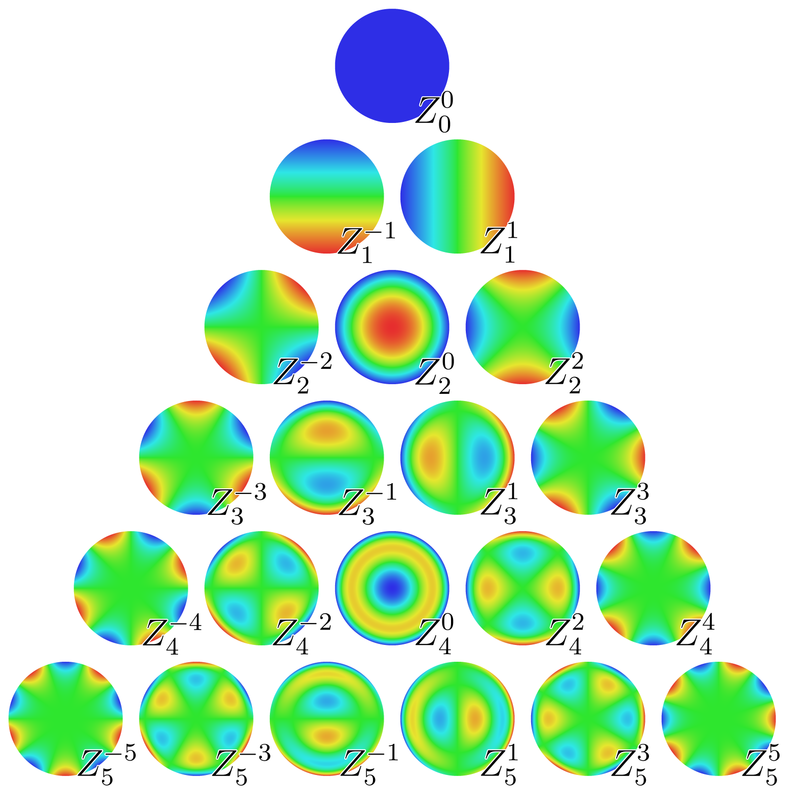
\includegraphics[width=0.60\textwidth]{nbar_MC/images/zernike}
     \caption{Zernike Polynomials representation. Moments $Z^0_4$ and $Z^1_5$ are widely discussed in this thesis}
\end{figure}

Precisely, Zernike Moments  $Z^0_4$ and $Z^1_5$ (\emph{clusterAbsZernikeMomen40} and \emph{clusterAbsZernikeMoment51} in the basf2 software) are studied in this thesis, where the first one represents the radial spread distribution structure, while the second one represents the level of dipolar asymmetry.

\paragraph{Number of Crystals hit}
$\\$
The variable Number of Crystals hit (\emph{clusterNhits} in the basf2 software) returns sum of weights $w_i$, with $w_i \le 1$ of all crystals in the cluster. For non-overlapping clusters this is equal to the number of crystals in the cluster. However, in the case of overlapping clusters where individual crystal energies are split among them, this can be a non-integer value.


